% This file provides an example Beamer presentation using the RWTH theme
% showcasing some of the more common options, similar to the Powerpoint version
% 12.11.2014: Revision 1 (Harold Bruintjes, Tim Lange)

% For RWTH, beamer should be loaded with class option t (top)
\documentclass[t]{beamer}


% Use fontspec to get Arial font
% Requires use of XeLaTeX
\usepackage{fontspec}
\setmainfont{Arial}
\setsansfont{Arial}
% Also force Arial for math for a more consistent look
\usepackage{unicode-math}
%\setmathfont{Arial}

% German style date formatting (footer)
\usepackage[ddmmyyyy]{datetime}
\renewcommand{\dateseparator}{.}

% Format the captions used for figures etc.
\usepackage[compatibility=false]{caption}
\captionsetup{singlelinecheck=off,justification=raggedleft,labelformat=empty,labelsep=none}

% PGFPlots is used for drawing some of the charts
\usepackage{pgfplots}
\pgfplotsset{compat=newest}
% This file contains some styles and macros for drawing charts similar to those of MS Office

\pgfplotsset{hor_barchart/.style={
  xbar=0mm,
  xmin=0,
  xtick=\empty,
  axis y line*=left,
  x axis line style={opacity=0},
  bar width=0.6cm,
  ytick=data,
  nodes near coords,
  every axis/.append style={font=\normalsize},
  every node near coord/.append style={font=\normalsize},
  nodes near coords align={horizontal},
  legend style={at={(0,-10mm)},anchor=north west,legend columns=-1,draw=none},
}}

\pgfplotsset{ver_barchart/.style={
  ybar=0mm,
  x = 4.5cm,
  ymin=0,
  ymajorgrids,
  axis x line*=bottom,
  y axis line style={opacity=0},
  bar width=0.8cm,
  enlarge x limits={0.15},
  xtick=data,
  nodes near coords,
  every axis/.append style={font=\normalsize},
  every node near coord/.append style={font=\normalsize},
  nodes near coords align={vertical},
  legend style={at={(0,-10mm)},anchor=north west,legend columns=-1,draw=none},
}}

\tikzstyle{chart}=[
    legend label/.style={font={\normalsize},anchor=west,align=left},
    legend box/.style={rectangle, draw=none, minimum size=5pt},
]

\tikzstyle{pie chart}=[
    chart,
    slice/.style={line cap=round, line join=round,draw=none},
    pie title/.style={font={\bf}},
    slice type/.style 2 args={
        ##1/.style={fill=##2},
        values of ##1/.style={}
    }
]

\newcommand{\pie}[3][]{
    \begin{scope}[#1]
    \pgfmathsetmacro{\curA}{90}
    \pgfmathsetmacro{\r}{1}
    \def\c{(0,0)}
    \node[pie title] at (90:1.3) {#2};
    \foreach \v/\s in{#3}{
        \pgfmathsetmacro{\deltaA}{\v/100*360}
        \pgfmathsetmacro{\nextA}{\curA + \deltaA}
        \pgfmathsetmacro{\midA}{(\curA+\nextA)/2}

        \path[slice,\s] \c
            -- +(\curA:\r)
            arc (\curA:\nextA:\r)
            -- cycle;

        %\begin{pgfonlayer}{foreground}
        % Position labels at 1.2 times radius (just outside of chart)
        \path \c -- node[pos=1.2,pie values,values of \s]{$\v\%$} +(\midA:\r);
        %\end{pgfonlayer}

        \global\let\curA\nextA
    }
    \end{scope}
}

% Custom legend (used for pie chart)
\newcommand{\legend}[2][]{
\begin{scope}[#1]
  \path
    \foreach \n/\s in {#2} {
      ++(0,-5pt) node[\s,legend box] {} +(5pt,0) node[legend label] {\n}
    };
\end{scope}
}


% Load the actual RWTH theme. Suggested is to load the full theme,
% as it requires some specific dimensions
\usetheme{rwth}

% Setup presentation information
\title{Interaktive Str\"omungssimulation}
\subtitle{Softwareentwicklungspraktikum}
\date[RWTH]{RWTH Symposium on LaTeX Beamer Templates\enskip|\enskip\today}
\author[Max]{Max Musterman mmusterman@rwth-aachen.de}
\institute[RWTH]{RWTH Aachen University}

% Set the logo to the file `logo`
% It will be scaled automatically
\logo{
\includegraphics{logo}}

% Uncomment this if you want a TOC at every section start
%\AtBeginSection{\frame{
%    \frametitle{Content}
%    \tableofcontents[currentsection]
%}}

% Use this to control some aspects of the footer
\setbeamertemplate{footertextextra}{Extra text in the footer\enskip|\enskip{}Extra text in the footer}
%\setbeamertemplate{footertext}{Example of an overridden footer}

\begin{document}

\setbeamertemplate{title page}[rwth]{}
\setbeamercolor{title page bar}{fg=white}
\setbeamertemplate{title page}[rwth3][unten]{}
\begin{frame}[plain]
\titlepage
\end{frame}


% Start a new section (text is displayed on top of a frame)
\section{Aufgabenstellung}
\subsection{Vorstellung}
% Frame with items
\begin{frame}{Aufgabe}
\begin{columns}[onlytextwidth]\
\begin{column}{.5\textwidth}
    Implementierung einer interaktiven echtzeit 2D Str\"omungssimulation von inkompressiblen Fluiden.
  \end{column}
  % Picture on the right
  \begin{column}{.5\textwidth}
    \raisebox{-5cm}[0cm][5cm]{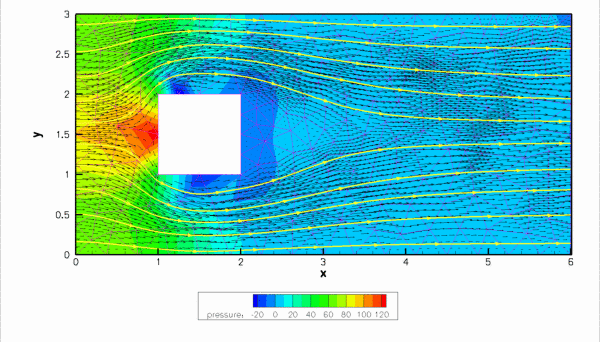
\includegraphics[width=10cm]{images/box_flow}}
  \end{column}
\end{columns}

\end{frame}

  \subsection{Anforderungen}

\begin{frame}{Bedingungen}
	Implementierung der inkompressiblen Navier-Stokes-Gleichung:
	\begin{itemize}
		\item C++
		\item Benutzeroberfl\"ache mit Qt
		\item Visualisierung mit OpenGL
		\item Echtzeitf\"ahige Randbedingungs\"anderung (z.B Hindernisse einzeichnen, Viskosit\"at \"andern)
		\item Verwendung verschiedener nummerischer Methoden
    \begin{itemize}
    \item Achtung: numerische Stabilit\"at
 	  \end{itemize}
 	  \item Lauff\"ahig auf dem RWTH-Cluster
    \item Minimale Hardware-Anforderungen
	\end{itemize}
\end{frame}

% Frame with text and picture
\subsection{Anwendungsfalldiagramm}
    
\begin{frame}{Anwendungsfalldiagramm}
  \begin{figure}[H]
	  \centering
	  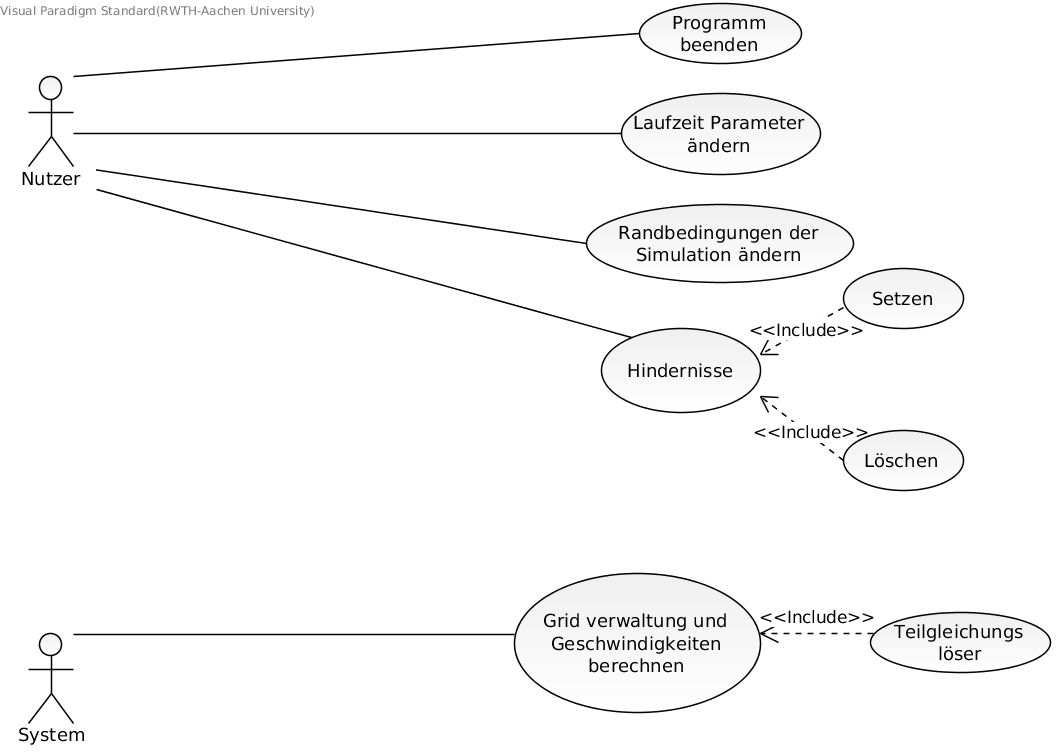
\includegraphics[height=0.7\textheight]{images/Strom-UCD}
	  \caption{Anwendungsfalldiagramm}
  \end{figure}
\end{frame}

\section{Mathematik}
  \subsection{Allgemein}

\begin{frame}{Navier-Stokes-Gleichung}
	\begin{align*}
	  \nabla \cdot \mathbf{u} &= 0
	  \\
	  \frac{\partial \mathbf{u}}{\partial t} &= - \left( \mathbf{u} \cdot \nabla \right) \mathbf{u} - \frac{1}{\rho} \nabla p + \nu \nabla^2 \mathbf{u} + \mathbf{f}
	\end{align*}

	\begin{itemize}
		\item \"Ubliches Diskretisieren mit FDM f\"uhrt bei gro{\ss}en Zeitschritten zu Instabilit\"at
			\begin{itemize}
			\item CFL-Zahl
			\end{itemize}
		\item Ansatz: Semi-Lagrangian scheme
	\end{itemize}
\end{frame}


\begin{frame}{Bedingungen}
	\begin{itemize}
	  \item Gestaffelt kartesisches Gitter
	  \item Verschiedene numerische Methoden
		\begin{itemize}
		\item Bedingungslose Stabilit\"at
		\end{itemize}
  \end{itemize}
\end{frame}

\begin{frame}{Gestaffelt kartesisches Gitter}
	\begin{itemize}
	  \item Vier Geschwindigkeiten
	  \item Ein Vektor mit Parametern
  \end{itemize}
    \begin{figure}[H]
	  \centering
	  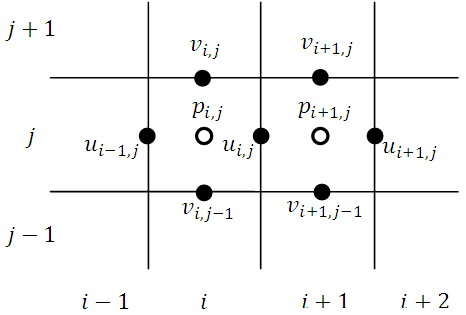
\includegraphics[width=0.6\textwidth]{images/grid}
	  \caption{Gestaffelt kartesisches Gitter}
  \end{figure}
\end{frame}

 \subsection{Navier-Stokes-Gleichung}
\begin{frame}{Navier-Stokes Teilgleichungen}
	Konvektionsterm mit Semi-Lagrangian scheme:
	\begin{align*}
	  \frac{\partial \mathbf{u}}{\partial t} &= \underbrace{\textcolor{red}{- \left( \mathbf{u} \cdot \nabla \right) \mathbf{u}}}_{\substack{Konvektion}} - \frac{1}{\rho} \nabla p + \nu \nabla^2 \mathbf{u} + \mathbf{f}
	\end{align*}
	\begin{itemize}
	\item  Particle Tracer (expliziter Euler oder Runge Kutta):
	\begin{itemize}
	\item  Bei jedem Zeitschritt: Berechne Ursprungspositionen aller Partikel.
	\end{itemize}
	\item Interpolation:
	\begin{itemize}
	\item Approximiert umliegende Gitterpunktwerte aller Partikel an dessen Ursprungspositionen.
	\end{itemize}
	\end{itemize}
\end{frame}


\begin{frame}{Navier-Stokes Teilgleichungen}
	Innere Kr\"afte durch Druck:
	\begin{align*}
	  \frac{\partial \mathbf{u}}{\partial t} &= - \left( \mathbf{u} \cdot \nabla \right) \mathbf{u} \underbrace{\textcolor{red}{- \frac{1}{\rho} \nabla p}}_{\substack{Druck}} + \nu \nabla^2 \mathbf{u} + \mathbf{f}
	\end{align*}
	\begin{itemize}
	\item  Lineares Verfahren, z.B Gauss Seidel
	\end{itemize}
\end{frame}

\begin{frame}{Navier-Stokes Teilgleichungen}
	Diffusionsterm:
	\begin{align*}
 	 \frac{\partial \mathbf{u}}{\partial t} &= - \left( \mathbf{u} \cdot \nabla \right) \mathbf{u} - \frac{1}{\rho} \nabla p + \underbrace{\textcolor{red}{\nu \nabla^2 \mathbf{u}}}_{\substack{Diffusion}} + \mathbf{f}
	\end{align*}
	\begin{itemize}
	\item  Implizites Euler Verfahren
	\end{itemize}
\end{frame}

\begin{frame}{Navier-Stokes Teilgleichungen}
	\"Aussere Kr\"afte:
	\begin{align*}
 	 \frac{\partial \mathbf{u}}{\partial t} &= - \left( \mathbf{u} \cdot \nabla \right) \mathbf{u} - \frac{1}{\rho} \nabla p + \nu \nabla^2 \mathbf{u} + \underbrace{\textcolor{red}{\mathbf{f}}}_{\substack{Kraft}}
	\end{align*}
	\begin{itemize}
	\item  Explizites Euler Verfahren
	\end{itemize}
\end{frame}

\section{Implementation}
  \subsection{Biblotheken}
  \begin{frame}{M\"oglichkeiten}
  \begin{block}{Entschieden}
    \begin{itemize}
      \item Mathematik: \textit{Eigen}
      \item Benutzeroberfl\"ache: \textit{QT 5.5 (wenn m\"oglich sonst 5.*)} 
      \item Eigentliche Str\"omung: \textit{OpenGl eingebettet in Qt}
    \end{itemize}
  \end{block}
  \begin{block}{Unentschlossen}
    \begin{itemize}
      \item Numerischeverfahren: \textit{odeint}
    \end{itemize}
  \end{block}
    \end{frame}
  \subsection{Aufteilung}
    \begin{frame}{Bibliothek, MVC}
    
  \begin{block}{Aufteilung}
    \begin{itemize}
      \item Benutzeroberfl\"ache: Model-View-Controller (MVC) (kein zusammen klicken)
      \item Solver: Reines C++ ohne Qt
    \end{itemize}
    \end{block}
    \begin{block}{Reihenfolge}
     \begin{itemize}
      \item Implimentierung von geg. Code und kartesischen Gitter
      \item \"Ubertragung auf Gestaffelten kartesischen Gitter
    \end{itemize}
    \end{block}
    
    \end{frame}
    \subsection{Demo}
    \begin{frame}{Demo}
    \hfill
      \center \raisebox{-4cm}[0cm][2cm]{\Huge{Demo}}
      \hfill
    \end{frame}

\end{document}
